% class
\documentclass[english, ngerman]{scrartcl}

% input preamble
\usepackage{iftex}

% text input and font
\ifluatex  % LuaLaTeX
    \usepackage{fontspec}
    % main font automatically: Latin Modern
    \IfFontExistsTF{Fira Code}{% true branch
        \setmonofont{Fira Code}[
            Contextuals=Alternate,  % Activate the calt feature
            StylisticSet={1,3,5,8}, % fontspec docs S. 46
            CharacterVariant={16}, % fontspec docs S. 37
            Numbers={SlashedZero} % fontspec docs S. 44
        ]}{% false branch
    }
\else  % pdfLaTeX
    \usepackage[utf8]{inputenc}  % input in UTF-8
    \usepackage[T1]{fontenc}  % output in T1 fonts (west European encoding)
    \usepackage{lmodern}  % Latin modern font for main text
    \IfFileExists{fira.sty}{% true branch
        \usepackage[mono]{fira}  % Fira (not Code!) font for monospaced text
    }{% false branch
    }
\fi

% text processing
\usepackage{babel}  % language package
\usepackage[intlimits]{mathtools}  % upgrade of amsmath (automatically loaded) - \int^_ like \limits^_
\usepackage{amssymb}  % upgrade of amsfonts (American Math Society)
\usepackage{amstext}  % \text command in math environments
\usepackage{letltxmacro}  % \let command for robust macros (new sqrt)
\usepackage{chemformula}  % typeset chemical formulas


% page geometry
\usepackage{scrlayer-scrpage}  % page formatting with KOMA options
\usepackage[paper=a4paper, hmargin=3cm, vmargin=2.5cm, includehead, includefoot]{geometry}  % horizontal: 3cm, vertical: 2.5cm strict with or without headers and footers
\usepackage{tabto}  % tab stops
\NumTabs{8}  % 8 equally spaced of \textwidth tab stops



% floats
\usepackage[hypcap=false, labelfont=bf]{caption, subcaption}  % caption editing - hypcap warning with hyperref
% counter prefixed with section number and therefore reset at each section:
\counterwithin{figure}{section}
\counterwithin{table}{section}
\usepackage{float}  % for [H] (forced here) specifier
\usepackage{tabularray}  % better tables
\usepackage{caption}  % better captions


% graphical input
\usepackage{graphicx}  % input JPEG, PNG, PDF, etc.
\usepackage{pdfpages}  % input PDF as whole pages
\usepackage{lastpage}  % reference to last page
\usepackage{import} % include files from other directories


% text
\usepackage[locale=DE, uncertainty-mode=separate]{siunitx}  % SI units, German formatting - \pm stays \pm instead of ..(.)
\let\sqty\qty  % physics overrides \qty of siunitx, therefore make it available as \sqty
\usepackage{physics}  % macros for easier typesetting of physical formulas
\usepackage{icomma}  % no space after commas instead of English points) in decimal values
\usepackage{enumitem}  % better enumerating with style options
\usepackage{nicefrac}  % inline-fractions in n/d-style
\usepackage{xcolor}  % custom colors
%TU-Graz colors
\definecolor{TUred}{HTML}{e4154b}
\definecolor{TUgray}{HTML}{bcbcbc}
\usepackage{listings, scrhack}  % code display; listings in combination with KOMA
\ifluatex
    \IfFontExistsTF{Fira Code}{%
        \usepackage[verbatim]{lstfiracode}  % Fira Code in listings
        \lstset{style=FiraCodeStyle}
    }{}
\fi
\usepackage{fancyvrb}  % Verbatim environment with better options (capital V!)


% literacy
\usepackage[sorting=none, giveninits=true]{biblatex}  % defaults: backend=Biber, style=numeric
% bibliography styles: https://www.overleaf.com/learn/latex/Biblatex_bibliography_styles
% citation styles: https://www.overleaf.com/learn/latex/Biblatex_citation_styles
\usepackage{csquotes}  % better quotation - should also be used in combination with package babel (warning)
\usepackage{xurl}  % breaks links - after BibLaTeX, but before hyperref!
\usepackage[hidelinks]{hyperref}  % produces most errors, last to load


% enumerate paragraphs and subparagraphs
% depths: https://www.overleaf.com/learn/latex/Sections_and_chapters
% -1 \part{part}
%  0 \chapter{chapter}
%  1 \section{section}
%  2 \subsection{subsection}
%  3 \subsubsection{subsubsection}
%  4 \paragraph{paragraph}
%  5 \subparagraph{subparagraph}
\setcounter{secnumdepth}{3}


% KOMA setups
% header and footer
\pagestyle{scrheadings}  % KOMA style
\clearpairofpagestyles  % reset
\setkomafont{pageheadfoot}{\normalfont}  % standard font in header and footer
\setlength{\headheight}{27.2pt}  % warning
\cfoot{\pagemark{} / \pageref*{LastPage}}  % center foot - *: ref but no hyperlink
% {}: empty statement
% \ : protected space
% \,: small space
\DeclareTOCStyleEntry[linefill=\TOCLineLeaderFill]{tocline}{section}  % sections in TableOfContents with dotted lines
% source: https://tex.stackexchange.com/a/651532
\KOMAoptions{parskip=half-}  % paragraphs with half a line height space instead of indentation, last line with no special treatment


% package setups

% rewrite names (babel overwrites German with standard English names, therefore at document beginn [after everything is loaded])
\AtBeginDocument{\renewcommand{\refname}{Literaturverzeichnis}}
% others:
% \contentsname
% \listtablename
% \listfigurename

% make title in bibliography upright
\DeclareFieldFormat{title}{#1}  % https://tex.stackexchange.com/a/311837
% make size of url in bibliography smaller
\renewcommand{\UrlFont}{\footnotesize\ttfamily}  % https://tex.stackexchange.com/a/151115, https://www.overleaf.com/learn/latex/Font_sizes%2C_families%2C_and_styles


% xcolor
\definecolor{code_keyword}{HTML}{A06E9D}
\definecolor{code_string}{HTML}{AD6E3E}
\definecolor{code_comment}{HTML}{6A9955}
% \definecolor{keyword_pink}{HTML}{c678dd}
% \definecolor{vscode_bg}{HTML}{282c34}
% \definecolor{vscode_var}{HTML}{e06c75}
% \definecolor{vscode_comment}{HTML}{7f848e}
% \definecolor{vscode_constant}{HTML}{d19a66}
% \definecolor{vscode_function}{HTML}{61afe3}
% \definecolor{background_grey}{HTML}{f8f8f8}
% \definecolor{code_basic}{HTML}{D4D4D4}
% \definecolor{code_background}{HTML}{1E1E1E}

% custom siunitx units
\DeclareSIUnit{\dig}{dig}  % digits for uncertainty of electronical measurement devices
\DeclareSIUnit{\px}{px}  % pixels
\sisetup{table-align-uncertainty=true}


% listings
\lstset{
    basicstyle=\ttfamily\footnotesize,%\color{code_basic},  % \footnotesize contains \selectfont implicitly
    %backgroundcolor=\color{code_background},
    commentstyle=\color{code_comment},
    keywordstyle=\bfseries\color{code_keyword},
    numberstyle=\tiny,
    stringstyle=\color{code_string},
    breakatwhitespace=false,
    breaklines=true,
    captionpos=b,
    keepspaces=true,
    numbers=left,
    numbersep=5pt,
    showspaces=false,
    showstringspaces=false,
    showtabs=false,
    tabsize=2
}


% new sqrt
% https://en.wikibooks.org/wiki/LaTeX/Mathematics
\makeatletter
\let\oldr@@t\r@@t
\def\r@@t#1#2{%
    \setbox0=\hbox{$\oldr@@t#1{#2\,}$}\dimen0=\ht0
    \advance\dimen0-0.2\ht0
    \setbox2=\hbox{\vrule height\ht0 depth -\dimen0}%
    {\box0\lower0.4pt\box2}}
\LetLtxMacro{\oldsqrt}{\sqrt}
\renewcommand{\sqrt}[2][\ ]{\oldsqrt[#1]{#2} }
\makeatother


% own commands
% \newcommand* can't contain multiple lines
% \newcommand can
\newcommand*{\mup}[1]{\ensuremath{\text{\textup{#1}}}}  % math mode upright normal font
\newcommand*{\inkgraphics}[3][\linewidth]{\def\svgwidth{#1}\import{#2}{#3}}
\newcommand{\todo}[1]{\textbf{\textcolor{TUred}{#1\\}}}


% custom tabularray environments

% imports and setups of tabularray: {
%     expl3,
%     xparse,
%     ninecolors
%     \hypersetup{pdfborder={0 0 0}}
% }

% additionally loaded libraries:
% diagbox
% varwidth
% booktabs
% counter

\UseTblrLibrary{amsmath}  % +array, +matrix, +bmatrix, +Bmatrix, +pmatrix, +vmatrix, +Vmatrix and +cases like tabularray with graphical options
\UseTblrLibrary{siunitx}  % siunitx suited for tabularray
\UseTblrLibrary{diagbox}  % table cells with diagonal lines, suited for tabularray
\UseTblrLibrary{varwidth}  % measure cell width
\UseTblrLibrary{booktabs}
\UseTblrLibrary{counter}


% custom tabularray environments:

% info:
% colcycle: https://github.com/lvjr/tabularray/issues/74
% guard: https://github.com/lvjr/tabularray/issues/175#event-6567229210

% guard S columns if latest feature ={guard} is not yet available
\newcommand*{\SiGuard}[1]{{#1}}

% standard environment
\SetTblrInner{
    hlines,
    vlines,
    columns={
            halign=c,
            valign=m,
        },
    measure=vbox,
}

% X columns
\NewTblrEnviron{tblrx}
\SetTblrInner[tblrx]{
    hlines,
    vlines,
    columns={
            halign=c,
            valign=m,
            co=1,  % coefficient of width for expendable columns (X columns)
        },
    width=\linewidth,
    vspan=minimal,
    measure=vbox,
}

% -X columns
\NewTblrEnviron{tblr-x}
\SetTblrInner[tblr-x]{
    hlines,
    vlines,
    columns={
            halign=c,
            valign=m,
            co=-1,  % shrinks X column down to natural width
        },
    width=\linewidth,
    vspan=minimal,
    measure=vbox,
}

% no hline and vline left and on top of first cell
\NewTblrEnviron{tblr_omit_first_cell}
\SetTblrInner[tblr_omit_first_cell]{
    hlines,
    vlines,
    columns={
            halign=c,
            valign=m,
        },
    hspan=even,
    vspan=minimal,
    %
    hline{1}={1}{white},  % first row, only first cell
    vline{1}={1}{white},
    measure=vbox,
}

% longtblr
\DefTblrTemplate{conthead-text}{default}{(Fortsetzung)}  % default: define and set at the same time
\DefTblrTemplate{contfoot-text}{default}{Fortsetzung auf nächster Seite}
\SetTblrStyle{caption-tag}{font=\bfseries}  % caption tag bold
\SetTblrInner[longtblr]{
    hlines,
    vlines,
    columns={
            halign=c,
            valign=m,
        },
    measure=vbox,
}

% longtblr - to adjust width of caption 
\DefTblrTemplate{firsthead}{default}{\addtocounter{table}{-1}\captionof{table}[\InsertTblrText{entry}]{\InsertTblrText{caption}}}
\DefTblrTemplate{middlehead,lasthead}{default}{\addtocounter{table}{-1}\captionof{table}[]{\InsertTblrText{caption}~(Fortsetzung)}}
%info ADD this to a local environment around the longtblr: \captionsetup{format=plain,labelfont=bf,font=small,  width=\linewidth}

% biblatex
\addbibresource{wirkungsgrad.bib}


% manual header
\ihead{Wirkungsgrad}  % inner (left) head
\chead{\textsc{Wachmann} Elias (12004232)\\\textsc{Zach} Andreas (12004790)}  % center head
\ohead{21.04.2023}  % outer (right) head

\newcommand{\FF}{\ensuremath{\mathit{FF}}}



\begin{document}

\begin{titlepage}
    \centering
    
\includegraphics[width=0.5\textwidth]{../../99_Misc/Logo_KF.pdf}\par\vspace{0.8cm}
    {\scshape\LARGE{Karl-Franzens-Universität Graz}\par}
    {\scshape\LARGE{Institut für Physik}\par}
    \vspace{1cm}
    {\scshape\Large{23S PHY.L02UB Fortgeschrittenenpraktikum 2}\par}
    678 Bachelorstudium Physik, UG2002/2021W\par
    \vspace{1.5cm}
    {\huge\bfseries III. Wirkungsgrad\par}
    \vspace{2cm}
    \begin{table}[H]
        \centering
        \begin{tabular}{c c c}
            \Large \textsc{Wachmann} Elias &  & \Large \textsc{Zach} Andreas \\
            \Large 12004232                &  & \Large 12004790              \\
            \multicolumn{3}{c}{Gruppe 12}
        \end{tabular}
    \end{table}
    \vfill
    \Large Betreut von\par
    Dr. Joachim \textsc{Krenn}
    \vfill
    {\large 21.04.2023\par}
\end{titlepage}

\clearpage
\tableofcontents
\newpage

\section[Aufgabenstellung]{Aufgabenstellung \cite{ref:angabe_solar,ref:angabe_waerme}}
\label{sec:aufgabenstellung}

\begin{itemize}
    \item Solarzelle
          \begin{itemize}
              \item Kennlinie und Kenndaten von Solarzellen in Parallel- und Serienschaltung bestimmen
              \item Aufnahme der Dunkel- und Hellkennlinie mittels Sonnensimulator
          \end{itemize}
    \item Wärmepumpe
          \begin{itemize}
              \item Messung des Temperaturverlaufes in zwei Wasserbehältern, der von der Pumpe aufgenommenen Leistung und der Drücke nach Kompression bzw. Expansion im Kältemittelkreislauf über \SI{30}{min}.
              \item Bestimmung der Leistungszahl und des Gütegrades als Funktion der Temperaturdifferenz.
              \item Erstellung des $p$-$H$-Diagrammes des Kreisprozesses aufgrund der gemessenen Werte zu Beginn und am Ende der Messung.
          \end{itemize}
\end{itemize}



\section[Voraussetzungen und Grundlagen]{Voraussetzungen und Grundlagen \cite{ref:angabe_solar,ref:angabe_waerme}}

\subsection{Solarzelle}
\label{subsec:grundlagen_solar}

\begin{figure}[H]
    \centering
    \begin{samepage}
        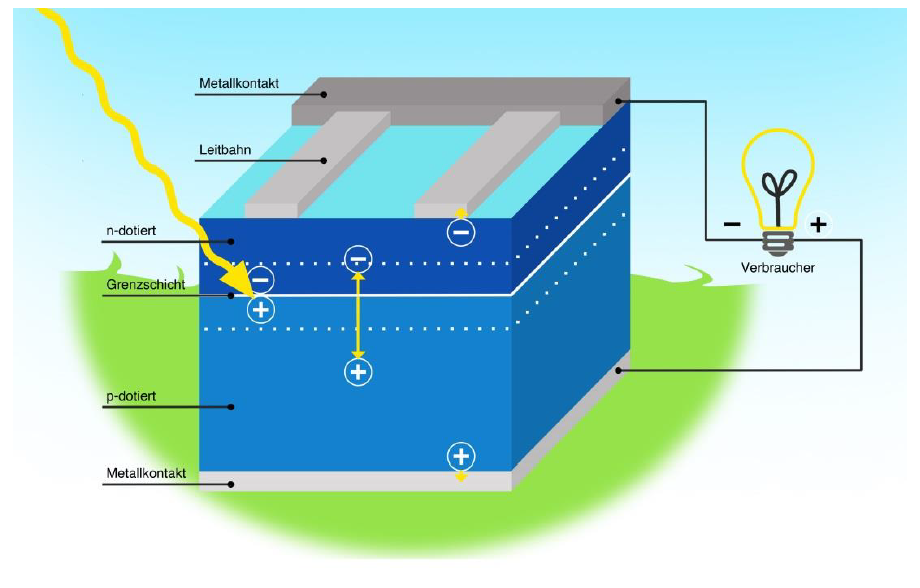
\includegraphics[width=0.7\linewidth]{fig/solarzelle_grundlagen.png}
        \caption{Schematischer Aufbau einer Solarzelle}
        \label{fig:solarzelle_schema}
    \end{samepage}
\end{figure}

Die Solarzelle besteht aus einer n-dotierten und einer p-dotierten Schicht, zwischen denen sich eine elektrisch neutrale Grenzschicht befindet. Die n-Schicht enthält als frei bewegliche Ladungsträger Elektronen, während die p-Schicht Elektronenlöcher aufweist. Die n-Schicht ist sehr dünn konstruiert, damit Sonnenlicht vor allem am p/n-Übergang absorbiert wird. Die p-Schicht dient der mechanischen Stabilität. Im vorliegenden Laborversuch werden monokristalline Siliziumsolarzellen verwendet. Die n-Schicht dieser Zellen wird durch oberflächennahes Einbringen von Phosphor-Atomen in das p-leitende Silizium-Substrat erzeugt, während die p-Schicht durch Dotieren mit Bor-Atomen entsteht. Die Fermi-Energie der n-Schicht wird dabei angehoben, jene der p-Schicht abgesenkt. Durch die unterschiedlichen Fermi-Niveaus wandern die Löcher in die n-Schicht und die Elektronen in die p-Schicht. Dadurch entsteht an der Grenzschicht eine von freien Ladungsträgern verarmte Sperrschicht. Durch diese Verschiebung der Ladungsträger bekommt das p-Gebiet eine negative, und das n-Gebiet eine positive Raumladung (Raumladungszone), welche das weitere Diffundieren der Ladungsträger verhindert. Erst durch Anlegen einer entgegengesetzten Spannung kann die entstandene Potentialbarriere abgebaut werden und Strom fließen. Wird eine äußere Spannung in umgekehrter Polarität angelegt, vergrößert sich die Potentialbarriere, die Sperrschicht dehnt sich weiter aus und kein Strom kann fließen. Damit verhält sich der p/n-Übergang als Gleichrichter und entspricht einer Diode. Wird die Sperrschicht mit Photonen einer genügend hohen Energie bestrahlt, so entstehen zusätzliche Elektron-Loch-Paare, welche die Energiebarriere überwinden können und ein Fotostrom in Sperrrichtung der Diode kann fließen. Aus der einfachen Diode ist dann eine Fotodiode geworden, welche als Solarzelle zur Stromerzeugung aus Strahlung verwendet werden kann.

Durch Ausmessen der Stromstärken zu in Durchlassrichtung angelegten Spannungen kann die $I$-$U$-Kennlinie der Diode	dargestellt werden. Per Konvention wird die Strom-Achse dabei invertiert dargestellt. Aus jener Kurve lassen sich Kenngrößen ablesen, wie etwa die Leerlaufspannung $U_L$ bei keinem Stromfluss oder der Kurzschlussstrom $I_K$ bei keiner angelegten Spannung. Die Leistung der Diode kann in Abhängigkeit von der Spannung über die Formel
%
\begin{equation}
    \label{eq:leistung}
    P = U \cdot I
\end{equation}
%
berechnet werden. Der Punkt maximaler Leistung $P_{\text{max}} = U_{\text{max}} \cdot I_{\text{max}}$ dient in Kombination mit der Leerlaufspannung und dem Kurzschlussstrom der Berechnung des Füllfaktors $\FF$
%
\begin{equation}
    \label{eq:fuellfaktor}
    \FF = \frac{U_{\text{max}} \cdot I_{\text{max}}}{U_L \cdot I_K}
\end{equation}
%
Dieser Faktor beschreibt das Verhältnis der rechteckigen Flächen bis zum Punkt maximaler Leistung und der aus Kurzschlussstrom und Leerlaufspannung aufgespanntem, was dem Energieverlust aufgrund der Kennlinienkrümmung entspricht. Dieser Zusammenhang ist in \autoref{fig:fuellfaktor} dargestellt.
%
\begin{figure}[H]
    \centering
    \begin{samepage}
        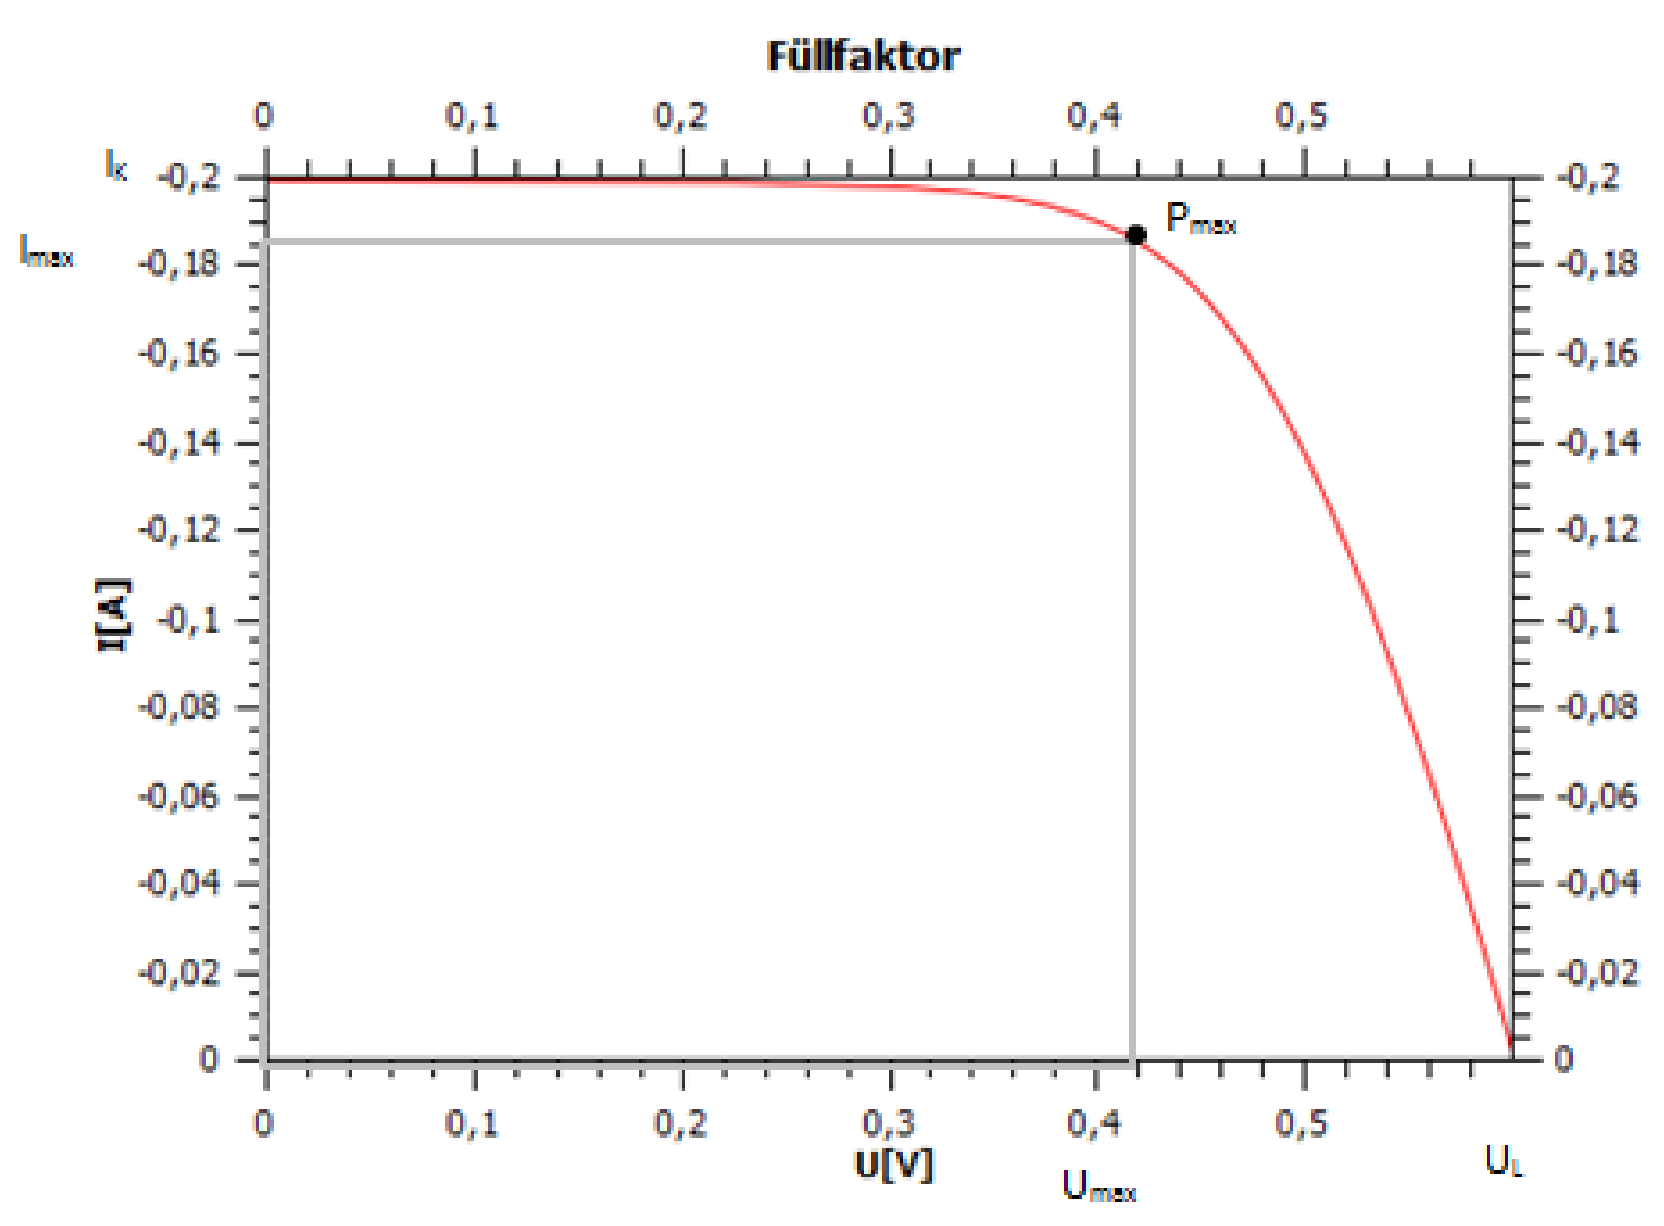
\includegraphics[width=0.7\linewidth]{fig/fuellfaktor.png}
        \caption[Füllfaktor]{Punkt maximaler Leistung im invertierten Strom-Spannung-Diagramm}
        \label{fig:fuellfaktor}
    \end{samepage}
\end{figure}

Im vorliegenden Laborversuch wird weiters die abgestrahlte Leistung eines Sonnensimulators berechnet. Hierzu skaliert man die auf der Solarzelle eintreffende Intensität $I_{\text{Licht}}$ mit ihrer aktiven Fläche $A = a \cdot b$, wobei $a$ und $b$ Länge respektive Breite der aktiven Fläche beschreiben. Setzt man die maximale Ausgangsleistung der Solarzelle $P_{\text{max}}$ in Relation zur einfallenden Lichtleistung $P_{\text{Licht}}$, erhält man den Wirkungsgrad $\eta$ des Gesamtsystems. Der Wirkungsgrad beschreibt, wie viel Eingangsleistung tatsächlich umgesetzt werden kann.
%
\begin{equation}
    \label{eq:wirkungsgrad}
    \eta = \frac{P_{\text{max}}}{P_{\text{Licht}}}
\end{equation}

Zur Bestimmung der Diodenparameter anhand der experimentell bestimmten $I$-$U$-Kurve wird die \textsc{Shockley}-Gleichung herangezogen.
Für einen idealisierten p/n-Übergang mit abruptem Dotierungsprofil erhält man als Strom-Spannungs-Charakteristik I(U) die Shockley-Gleichung:
%
\begin{equation}
    \label{eq:shockley}
    I(U) = I_S \cdot \left( e^{\frac{q_e U}{k_B T}} - 1 \right)
\end{equation}
%
Dabei beschreibt $U$ die an der Diode angelegte Spannung (positiv in Durchlassrichtung, negativ in Sperrrichtung), $I_S$ den Sättigungsstrom, $T$ die Temperatur, $k_B$ die Boltzmann-Konstante und $q_e$ die Elementarladung. Dieses idealisierte Verhalten ist
meist in der Praxis nicht gegeben, weshalb man für eine reale Diode den Diodenfaktor $f$ einführt.
Wird die Sperrschicht zusätzlich beleuchtet, so entstehen Elektron-Loch-Paare, welche einen Fotostrom $I_{\text{ph}}$ in Sperrrichtung verursachen. Aus der Shockley-Gleichung erhält man dann für eine beleuchtete Fotodiode:
%
\begin{equation}
    \label{eq:shockley_beleuchtet}
    I(U) = I_S \cdot \left( e^{\frac{q_e U}{f k_B T}} - 1 \right) - I_{\text{ph}}
\end{equation}


\subsection{Wärmepumpe}
\label{subsec:grundlagen_waermepumpe}

Eine Wärmepumpe ist eine thermodynamische Maschine, die einen Kreisprozess realisiert. Ein Arbeitsmedium (hier das Kältemittel R-134a) durchläuft vier Schritte. Zuerst wird es vom Kompressor vom Druck $p_1$ auf den Druck $p_2$ adiabatisch komprimiert. Dabei erwärmt sich
das Arbeitsmedium auf die Temperatur $T_k$. Das Arbeitsmedium gibt dann über einen Wärmetauscher isobar Wärme an den Körper höherer Temperatur ab und wird annähernd auf dessen Temperatur $T_2$ abgekühlt, wobei es kondensiert. Danach wird das Arbeitsmedium
anhand eines Ventils auf den niedrigeren Druck $p_1$ entspannt, wobei es erkaltet. Das nun kalte, ensptannte Arbeitsmedium nimmt dann über einen zweiten Wärmetauscher isobar Wärme vom Körper niedrigerer Temperatur auf und erwärmt sich dabei auf annähernd dessen Temperatur $T_1$, wobei es wieder verdampft. Nun beginnt der Kreisprozess von vorne. Durch diesen Vorgang
wird dem kalten Reservoir ($T_1$) Wärme entzogen und dem warmen ($T_2$) zugefügt. Zusammengefasst besteht der idealisierte Kreisprozess aus einer adiabatischen Kompression, einer isobaren Abkühlung, einer isenthalpen Expansion und einer isobaren Erwärmung.

Zur Bewertung der Leistungsfähigkeit des Kreisprozesses wird die Leistungszahl $\epsilon$ eingeführt. Diese ist definiert als das Verhältnis des dem Reservoir $T_2$ durch die Pumpe zugeführten Wärmestroms $\dot{Q}$ (Wärmemenge $\Delta Q$ pro Zeiteinheit $\Delta t$) zur aufgenommenen Leistung $P$ des Kompressors:
%
\begin{equation}
    \label{eq:leistungszahl}
    \epsilon = \frac{\dot{Q}}{P}
\end{equation}
%
Der Wärmestrom $\dot{Q}$ lässt sich dabei nach der folgenden Formel berechnen:
%
\begin{equation}
    \label{eq:waermestrom}
    \dot{Q} = c \cdot m \cdot \dot{T},
\end{equation}
%
wobei $c$ die spezifische Wärmekapazität von Wasser und $m$ die Masse des Wassers darstellt. Man definiert nun noch den Gütegrad $\eta$ einer Wärmepumpe als Verhältnis der Leistungszahl $\epsilon$ der Wärmepumpe zur theoretisch maximal erreichbaren Leistungszahl, der Leistungszahl des Carnot-Prozesses $\epsilon_{\text{max}} = \frac{T_2}{T_2-T_1}$.
%
\begin{equation}
    \label{eq:guetegrad}
    \eta = \frac{\epsilon}{\epsilon_{\text{max}}}
\end{equation}



\section{Versuchsanordnung}
\label{sec:versuchsanordnung}

Das vorliegende Labor teilt sich in zwei Teilversuche auf, welchen Aufbau in den folgenden Abschnitten beschrieben wird.

\subsection{Solarzelle}
\label{subsec:anordnung_solarzelle}

Der Versuch zur Solarzelle teilt sich nun weiter in zwei Aufbauten ein. Der erste der beiden ist in \autoref{fig:solar_aufbau} dargestellt. Dabei wird der Aufbau, wie in \cite{ref:angabe_solar} beschrieben, realisiert. Die Lichtquelle, die Lampe rechts im Bild, wird hierzu \SI{30}{cm} von den beiden Solarzellen entfernt positioniert. Ein variabler Widerstand fungiert als Last und die Messung wird wie nachfolgend beschrieben mit zwei Multimetern, jeweils für eine serielle als auch parallele Schaltung der beiden Solarmodule, durchgeführt.
%
\begin{figure}[H]
    \centering
    \begin{samepage}
        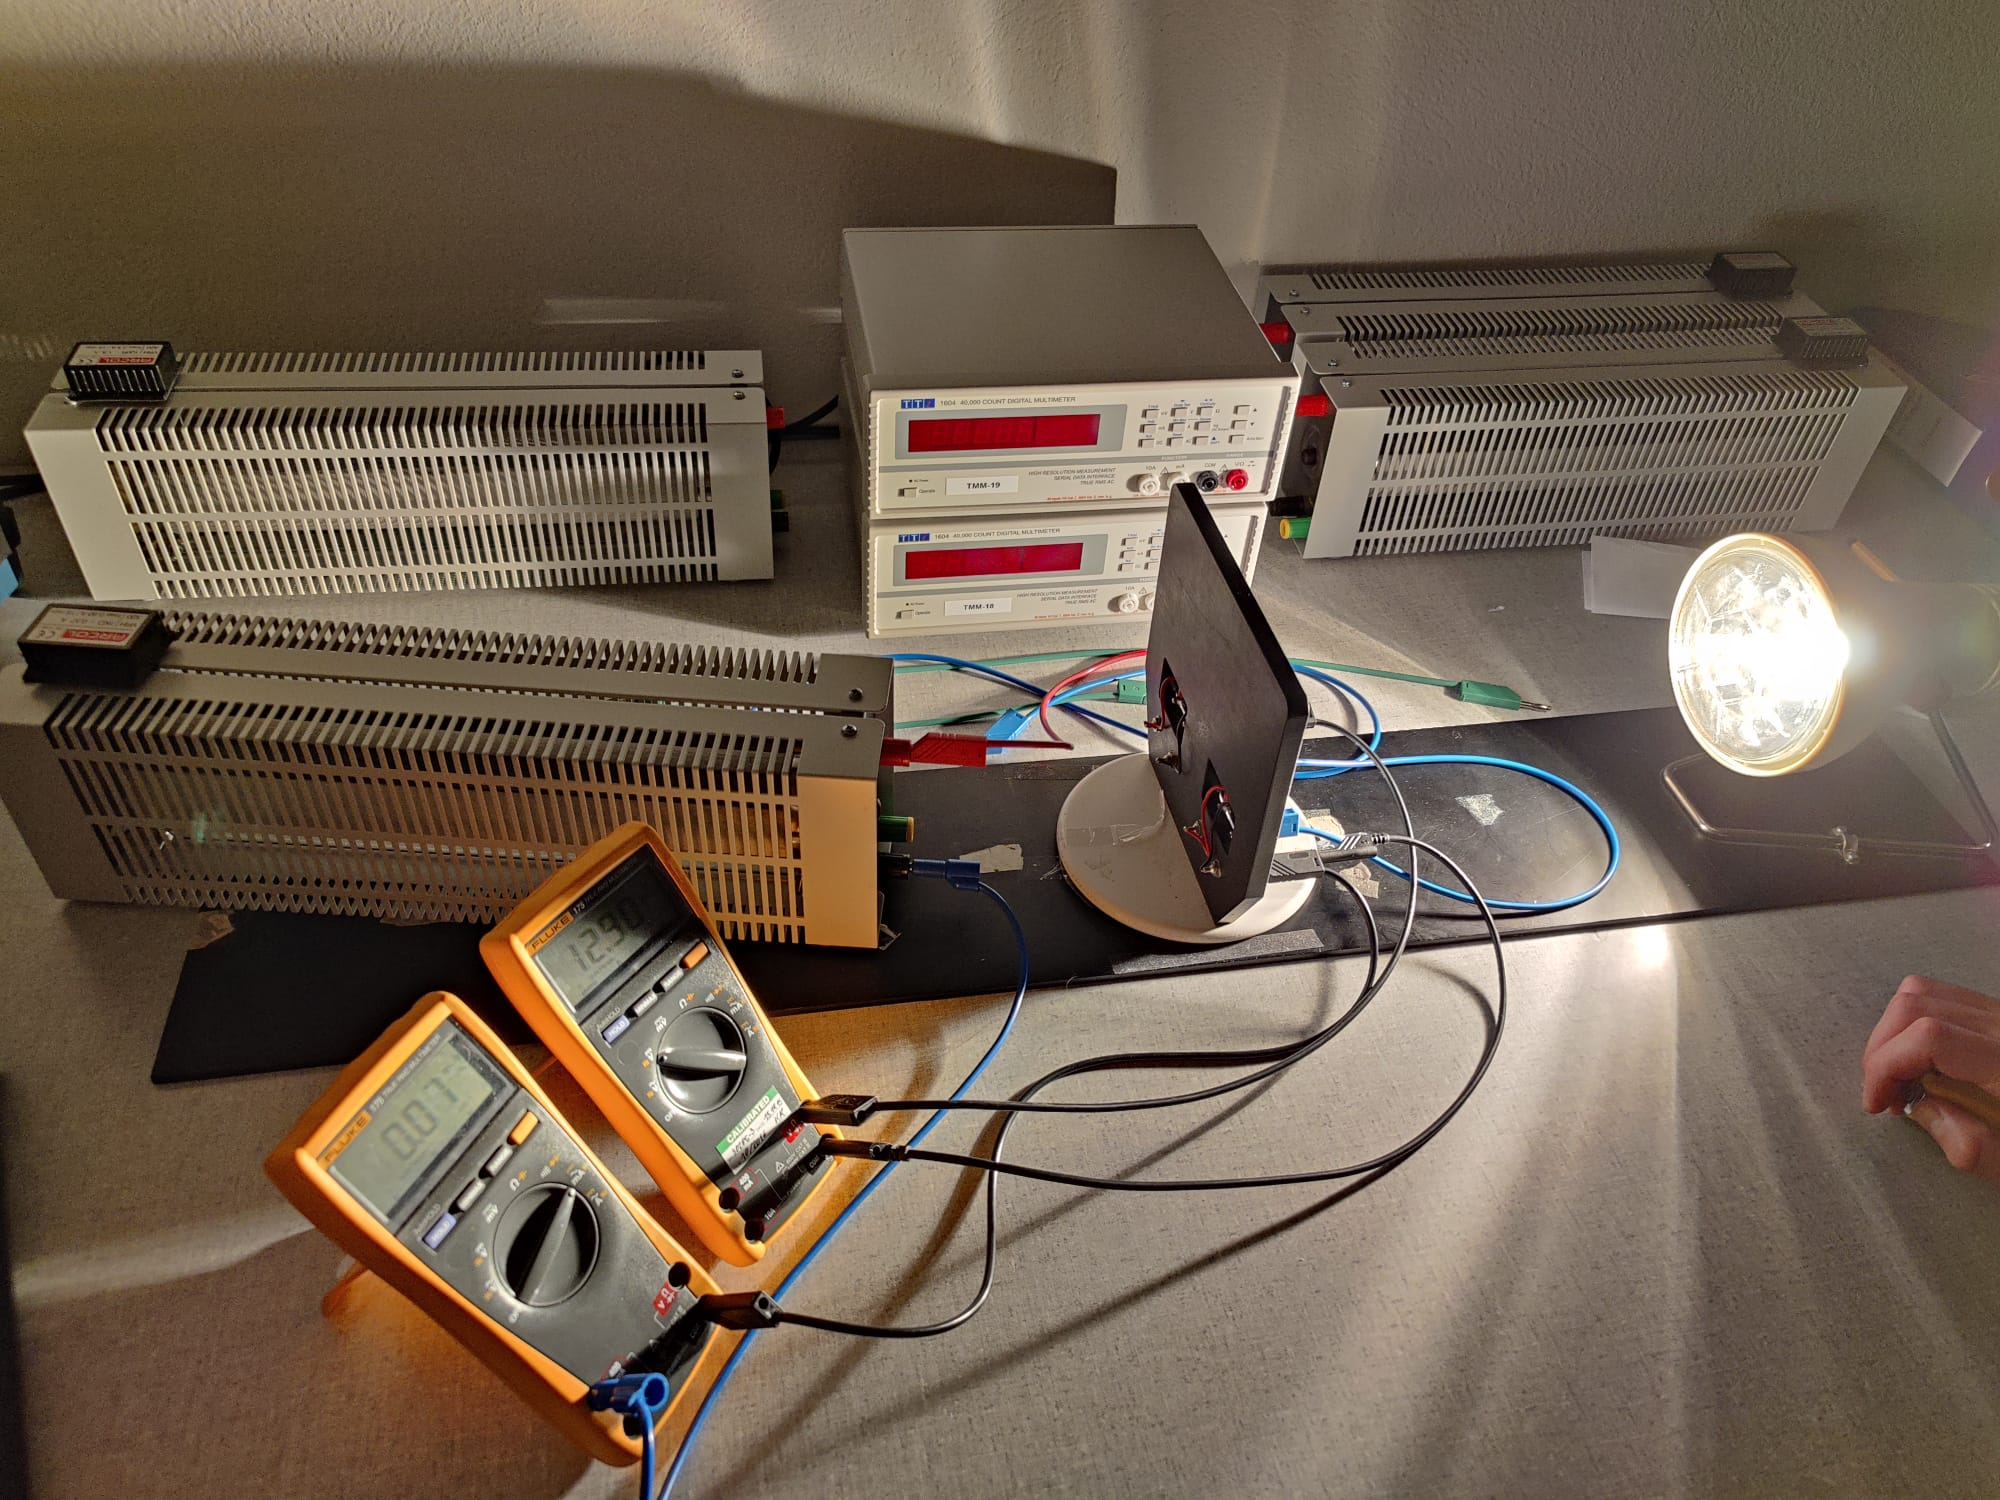
\includegraphics[width=0.6\linewidth]{fig/Aufbau_solar.jpeg}
        \caption[Aufbau Kennlinie Solarzelle Lampe]{Aufbau des Versuchs zur Bestimmung der Kennlinie einer Solarzelle.}
        \label{fig:solar_aufbau}
    \end{samepage}
\end{figure}
%
Für den zweiten Aufgabenteil wird nun auf den zweiten Versuchsaufbau gewechselt. Hier steht ein Sonnensimulator (rechts in \autoref{fig:sonne_aufbau}) zur Verfügung. Dieser ist in der Lage eine gewisse konstante Lichtintensität zu erzeugen, welche auf die Solarzelle trifft. Letztere ist an ein Sourcemeter angeschlossen, welches automatisiert die Kennlinienauffzeichnung durchführt. Die Lichtintensität wird vor der Aufzeichung noch mittels Powermeter gemessen.
%
\begin{figure}[H]
    \centering
    \begin{samepage}
        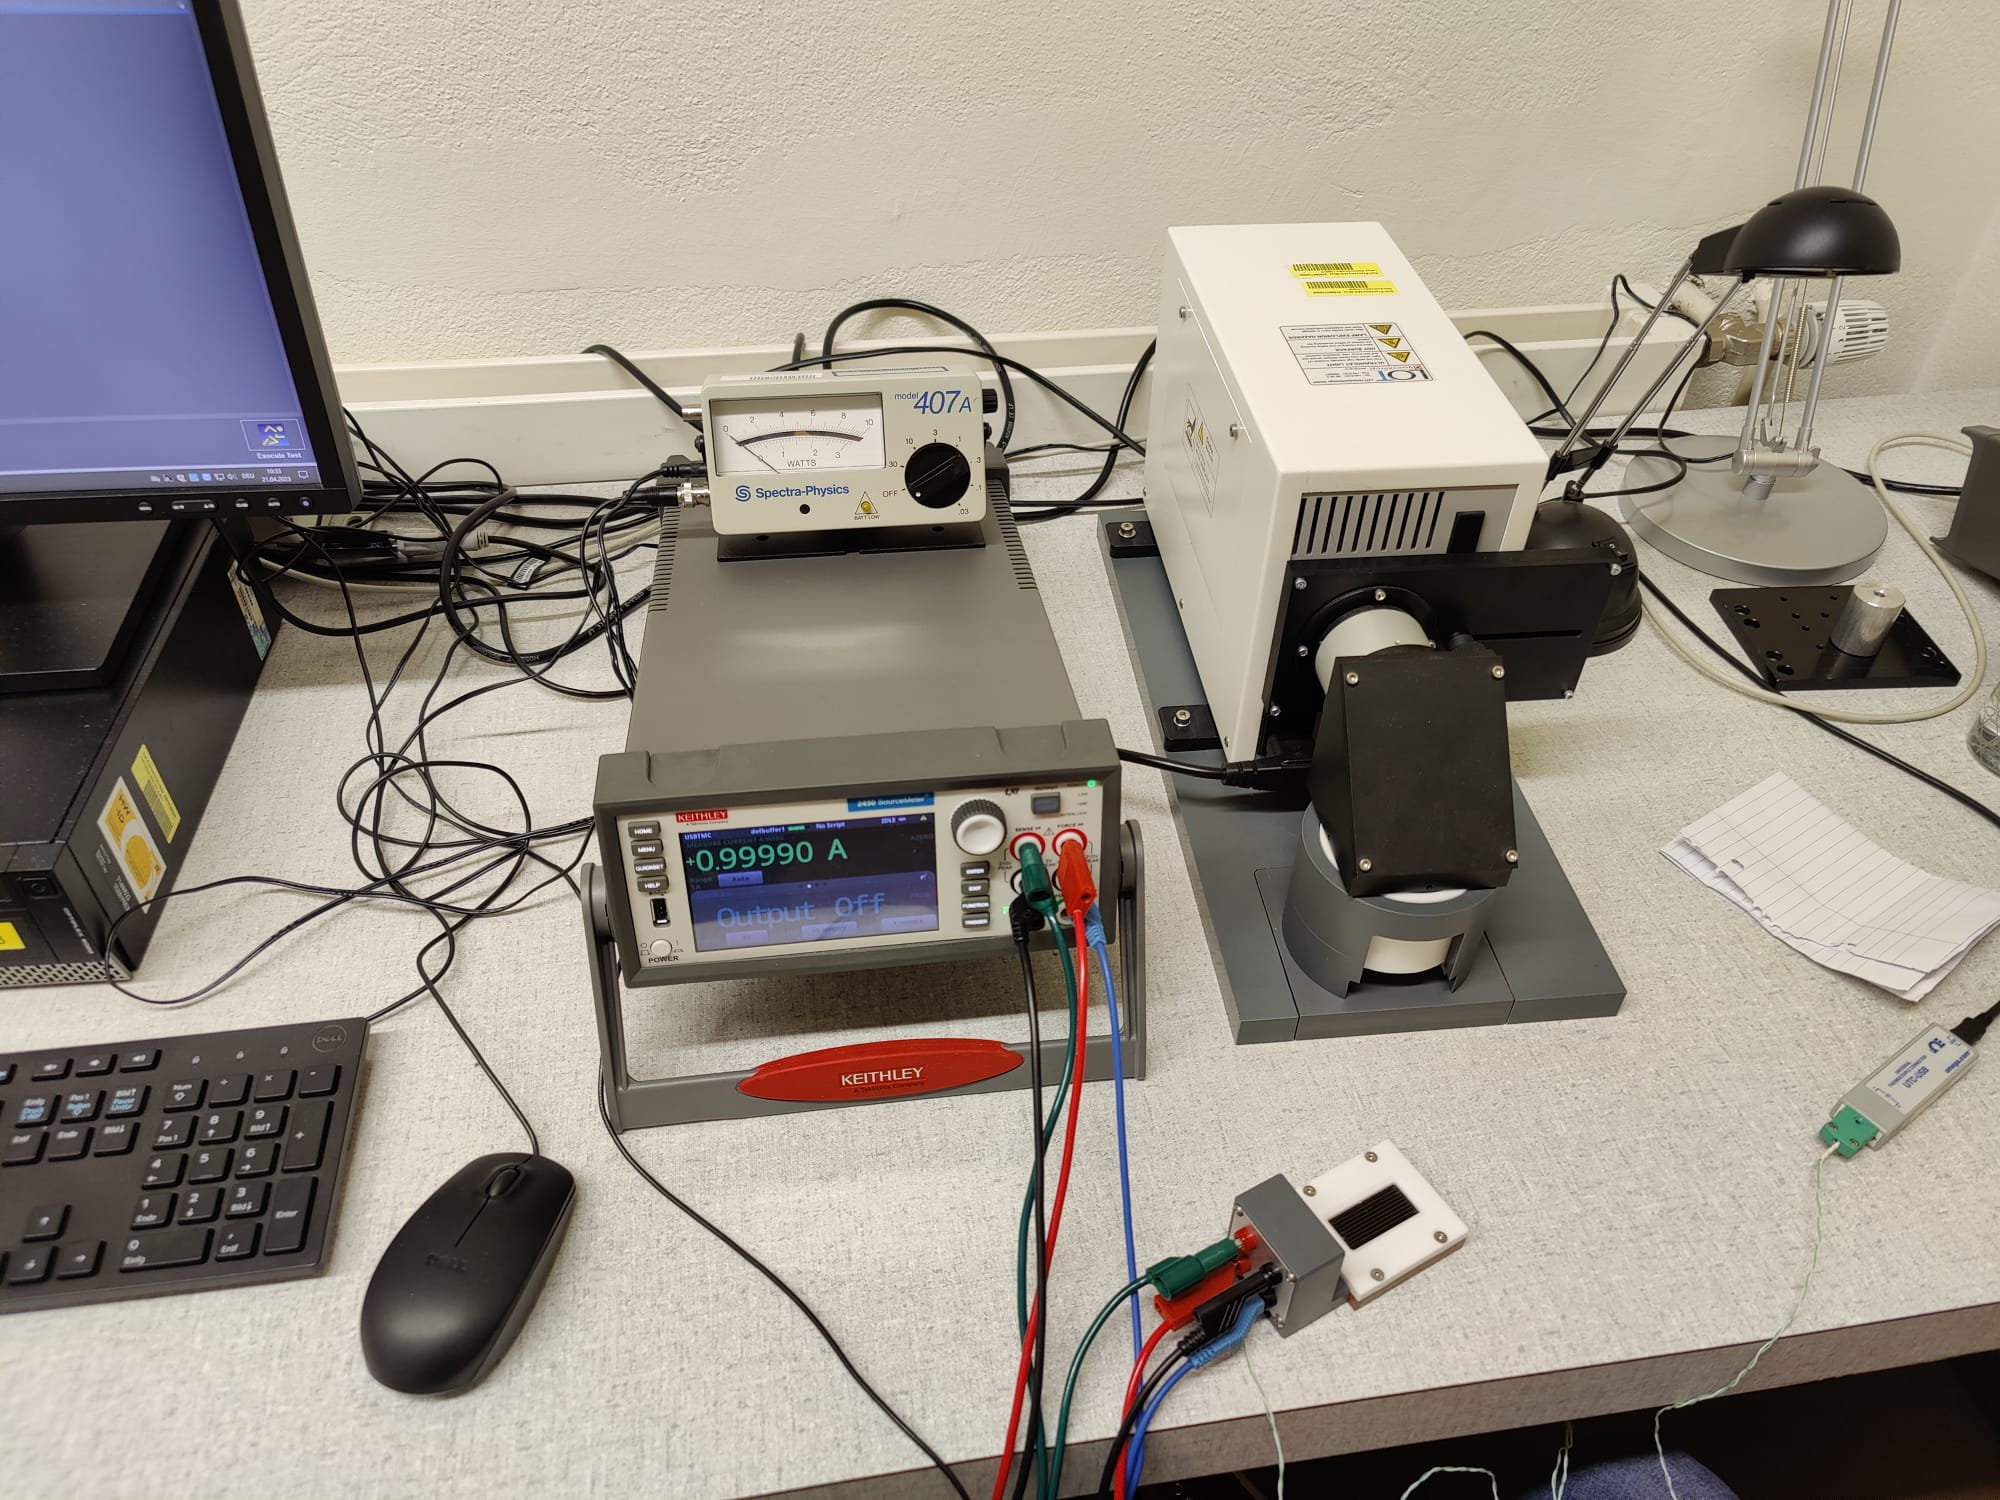
\includegraphics[width=0.6\linewidth]{fig/Aufbau_Sonnensimulator.jpeg}
        \caption[Aufbau Hell- und Dunkelkennlinie Solarzelle Sonnensimulator]{Aufbau des Versuchs zur Bestimmung der Dunkel- und Hellkennlinie mittels Sonnensimulator}
        \label{fig:sonne_aufbau}
    \end{samepage}
\end{figure}


\subsection{Wärmepumpe}
\label{subsec:anordnung_waermepumpe}

Für den Versuch zur Wärmepumpe wird der bereits aufgebaute Versuch, schematisch in \autoref{fig:waerme_aufbau} dargestellt, verwendet. Lediglich die Temperaturmessgeräte werden noch mittels Cassy Lab2 Schnittstelle mit dem nebenstehenden Computer verbunden.
%
\begin{figure}[H]
    \centering
    \begin{samepage}
        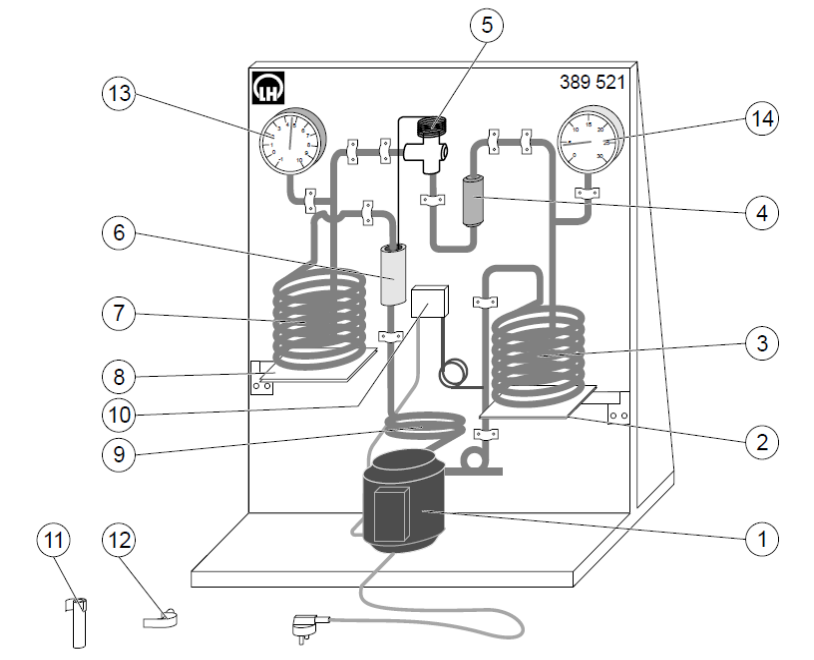
\includegraphics[width=0.8\linewidth]{fig/Waermepumpe_schematisch.png}
        \caption[Schematischer Aufbau Wärmepumpe]{Versuchsaufbau. \textbf{1:} Kompressor \SI{230}{V}, \SI{50}{Hz} oder \SI{60}{Hz}. Leistungsaufnahme ca. \SI{130}{W} bei \SI{50}{Hz}; \textbf{2:} ausschwenkbare Stellfläche für rot-markierten Warmwasserbehälter; \textbf{3:} Verflüssiger; \textbf{4:}
            Sammler/Reiniger; \textbf{5:} Expansionsventil; \textbf{6:} Temperaturfühler des Expansionsventils; \textbf{7:} Verdampfer; \textbf{8:} ausschwenkbare Stellfläche Kaltwasserbehälter; \textbf{9:} Rohrwindungen als elastische Verbindung zwischen Kompressor und Wärmetauscher; \textbf{10:} Druckwächter; \textbf{11:} Kunststoffhalter ($2\times$) für
            Thermometer und Temperaturfühler, zum Anklemmen an Kupferrohre; \textbf{12:} Kupfer-Messschuh ($2\times$)
            zum Einstecken von Temperaturfühlern für Temperaturmessungen an den Kupferrohren des Kältemittelkreislaufs; \textbf{13:} Manometer für die Niederdruckseite; innere Skala für Druckmessung von \SIrange{-1}{10}{\bar}, äußerste Skala mit zugehöriger Taupunkttemperatur für R-134a von \SIrange{-60}{40}{\celsius};
            \textbf{14:} Manometer für die Hochdruckseite; innere Skala: Druck von \SIrange{-1}{30}{\bar}, äußerste Skala mit
            zugehöriger Taupunkttemperatur für R-134a von \SIrange{-60}{85}{\celsius} \cite{ref:angabe_waerme}.}
        \label{fig:waerme_aufbau}
    \end{samepage}
\end{figure}



\section{Geräteliste}
\label{sec:geraeteliste}

\begin{table}[H]
    \centering
    \begin{samepage}  % caption and table on same page
        \caption[Geräteliste]{Verwendete Geräte und wichtige Materialien}  % optional argument for List of Tables, mandatory argument for caption
        \label{tab:geraeteliste}
        \begin{tblrx}{row{1}={guard}}
            Gerät                     & Modell               & Inv. Nummer  & Anmerkung                         \\
            $2\times$ Solarzelle      & -                    & -            & -                                 \\
            Lampe                     & -                    & -            & -                                 \\
            Multimeter                & Fluke 175 True RMS   & -            & -                                 \\
            Widerstand                & variabel             & -            & -                                 \\
            Sourcemeter               & Keithley 2450        & 310084940000 & -                                 \\
            Powermeter                & Spectra-Physics 407A & 310041630000 & -                                 \\
            Sonnensimulator           & -                    & 310094110000 & -                                 \\
            PC mit Kickstart Software & -                    & -            & -                                 \\
            Wärmepumpenaufbau         & -                    & 310070540000 & siehe \autoref{fig:waerme_aufbau} \\
            Eimer                     & \SI{5}{\liter}       & -            & -                                 \\
            Temperaturmessgeräte      & -                    & 666206       & -                                 \\
            PC mit Cassy Lab2         & -                    & -            & -                                 \\
        \end{tblrx}
    \end{samepage}
\end{table}



\section{Versuchsdurchführung und Messergebnisse}
\label{sec:versuchsdurchfuehrung_messergebnisse}

\subsection{Solarzelle mit Lampe}
\label{subsec:durchfuehrung_solar_lampe}
%? Disclaimer: Hamma das mit der Abdeckung der einen Solarzelle falsch gemacht? Mir kommt vor, wir haben eine der beiden vollständig abgedeckt, wir hätten die aber, glaub ich, nur teilweise abdecken sollen.
Der Aufbau wird, wie in \autoref{subsec:anordnung_solarzelle} beschrieben und in \autoref{fig:solar_aufbau} dargestellt, aufgebaut. Der Abstand zwischen Lampe und Solarzellenmodulen beträgt circa \SI{30}{cm}. Nacheinander werden nun insgesamt drei Variatonen desselben Aufbaus experimentell behandelt. Zuerst werden die beiden Solarzellenmodule in Serie geschaltet, anschließend parallel und zu guter Letzt wieder in Serie, diesmal wird jedoch ein Modul gänzlich von Lichteinfall abgeschirmt.

Zu Beginn wird der Schiebewiderstand auf seinen Maximalwert von \SI{1}{\kilo\ohm} eingestellt. Stückweise wird nun der Widerstandswert verringert indem die gesamte Bandbreite des variablen Widerstands ausgenutzt wird, um die Strom-Spannungskennlinie der Solarzelle bestimmen zu können. Bei jeder neuen Position des Schiebers (und damit neuem Widerstandswert) werden sowohl Strom als auch Spannung an Ampere- bzw. Voltmeter abgelesen und notiert. Im Bereich des annähernd linearen Verlaufs der Kurve werden großzügigere Widerstandswertschritte gewählt, im interessanten Bereich des Punkts der maximalen Leistung werden kleinere Schrittweiten am Widerstand gewählt. Die erhaltenen Messwerte für Strom und Spannung im seriellen Aufbau finden sich in \autoref{tab:messergebnisse_solar_seriell}.
%
\begin{table}[H]
    \centering
    \begin{samepage}
        \caption[Messergebnisse Solarzelle seriell]{Gemessene Ströme $I$ und Spannungen $U$ der beiden Solarzellenmodule in Serienschaltung zur Bestimmung der Kennlinie der Zelle. Der Verbraucherwiderstand wird mittels variablem Schiebewiderstand ($R_{\text{max}}=\SI{1}{\kilo\ohm}$) laufend verändert. Unsicherheiten laut Fluke-Datenblatt.}
        \label{tab:messergebnisse_solar_seriell}
        \begin{tblr}{colspec={S[table-format=2.2]S[table-format=1.2]S[table-format=2.4]S[table-format=1.4]}, row{1}={guard}}
            $I$ / \si{mA} & $\Delta I$ / \si{mA} & $U$ / \si{V} & $\Delta U$ / \si{V} \\
            0.00          & 0.03                 & 11.65        & 0.02                \\
            11.70         & 0.15                 & 11.48        & 0.02                \\
            15.19         & 0.19                 & 11.40        & 0.02                \\
            19.8          & 0.3                  & 11.300       & 0.019               \\
            24.2          & 0.3                  & 11.200       & 0.019               \\
            26.6          & 0.3                  & 11.150       & 0.019               \\
            28.9          & 0.4                  & 11.100       & 0.019               \\
            30.9          & 0.4                  & 11.060       & 0.019               \\
            34.0          & 0.4                  & 10.980       & 0.019               \\
            38.5          & 0.5                  & 10.860       & 0.019               \\
            43.5          & 0.5                  & 10.720       & 0.019               \\
            48.4          & 0.6                  & 10.550       & 0.018               \\
            52.0          & 0.6                  & 10.390       & 0.018               \\
            54.5          & 0.6                  & 10.240       & 0.018               \\
            55.6          & 0.6                  & 10.140       & 0.018               \\
            56.6          & 0.6                  & 9.940        & 0.017               \\
            57.1          & 0.7                  & 9.810        & 0.017               \\
            57.2          & 0.7                  & 9.670        & 0.017               \\
            57.3          & 0.7                  & 9.550        & 0.017               \\
            57.3          & 0.7                  & 9.400        & 0.017               \\
            57.2          & 0.7                  & 9.340        & 0.017               \\
            57.3          & 0.7                  & 8.980        & 0.016               \\
            57.8          & 0.7                  & 7.770        & 0.014               \\
            58.2          & 0.7                  & 6.250        & 0.012               \\
            58.7          & 0.7                  & 5.490        & 0.011               \\
            59.5          & 0.7                  & 4.310        & 0.009               \\
            61.2          & 1.0                  & 2.720        & 0.007               \\
            63.3          & 1.0                  & 0.690        & 0.004               \\
            65.5          & 1.0                  & 0.1200       & 0.0004              \\
            65.4          & 1.0                  & 0.0000       & 0.0002              \\
        \end{tblr}
    \end{samepage}
\end{table}
%
Anschließend werden die beiden Solarzellenmodule parallel verbunden und eine erneute Messserie wird dokumentiert. Die Messergebnisse finden sich in \autoref{tab:messergebnisse_solar_parallel}.
\begin{table}[H]
    \centering
    \begin{samepage}
        \caption[Messergebnisse Solarzelle parallel]{Gemessene Ströme $I$ und Spannungen $U$ der beiden Solarzellenmodule in Parallelschaltung zur Bestimmung der Kennlinie der Zelle. Der Verbraucherwiderstand wird mittels variablem Schiebewiderstand ($R_{\text{max}}=\SI{1}{\kilo\ohm}$) laufend verändert. Unsicherheiten laut Fluke-Datenblatt.}
        \label{tab:messergebnisse_solar_parallel}
        \begin{tblr}{colspec={S[table-format=3.2]S[table-format=1.2]S[table-format=1.4]S[table-format=1.4]}, row{1}={guard}}
            $I$ / \si{mA} & $\Delta I$ / \si{mA} & $U$ / \si{V} & $\Delta U$ / \si{V} \\
            0.00          & 0.03                 & 5.793        & 0.011               \\
            5.98          & 0.09                 & 5.850        & 0.011               \\
            7.82          & 0.11                 & 5.834        & 0.011               \\
            9.34          & 0.13                 & 5.820        & 0.011               \\
            11.49         & 0.15                 & 5.810        & 0.011               \\
            13.28         & 0.17                 & 5.796        & 0.011               \\
            18.6          & 0.3                  & 5.765        & 0.011               \\
            28.0          & 0.4                  & 5.710        & 0.011               \\
            36.2          & 0.4                  & 5.660        & 0.011               \\
            45.7          & 0.5                  & 5.602        & 0.011               \\
            53.7          & 0.6                  & 5.552        & 0.011               \\
            60.6          & 1.0                  & 5.507        & 0.011               \\
            67.1          & 1.0                  & 5.460        & 0.011               \\
            70.7          & 1.1                  & 5.438        & 0.011               \\
            78.6          & 1.1                  & 5.386        & 0.011               \\
            91.2          & 1.3                  & 5.295        & 0.010               \\
            98.1          & 1.3                  & 5.245        & 0.010               \\
            111.0         & 1.5                  & 5.145        & 0.010               \\
            127.4         & 1.6                  & 5.000        & 0.010               \\
            141.8         & 1.8                  & 4.850        & 0.010               \\
            150.2         & 1.9                  & 4.770        & 0.010               \\
            169           & 2                    & 4.480        & 0.009               \\
            184           & 3                    & 3.850        & 0.008               \\
            185           & 3                    & 1.500        & 0.005               \\
            189           & 3                    & 0.0200       & 0.0003              \\
            189           & 3                    & 0.0000       & 0.0002              \\
        \end{tblr}
    \end{samepage}
\end{table}
%
Zu guter Letzt wird die Anordnung wieder seriell verschaltet und eine der beiden Zellen mittels mehreren Blättern Papiers vor einfallendem Licht abgeschirmt. Die Messergebnisse finden sich in \autoref{tab:messergebnisse_solar_seriell_abgeschirmt}.
%
\begin{table}[H]
    \centering
    \begin{samepage}
        \caption[Messergebnisse Solarzelle seriell]{Gemessene Ströme $I$ und Spannungen $U$ der beiden Solarzellenmodule in Serienschaltung, wobei eine der beiden Zellen vor dem einfallenden Licht abgeschirmt ist, zur Bestimmung der Kennlinie der Zelle. Der Verbraucherwiderstand wird mittels variablem Schiebewiderstand ($R_{\text{max}}=\SI{1}{\kilo\ohm}$) laufend verändert. Unsicherheiten laut Fluke-Datenblatt.}
        \label{tab:messergebnisse_solar_seriell_abgeschirmt}
        \begin{tblr}{colspec={S[table-format=1.2]S[table-format=1.2]S[table-format=2.4]S[table-format=1.4]}, row{1}={guard}}
            $I$ / \si{mA} & $\Delta I$ / \si{mA} & $U$ / \si{V} & $\Delta U$ / \si{V} \\
            0.00          & 0.03                 & 10.100       & 0.018               \\
            2.93          & 0.06                 & 2.860        & 0.007               \\
            2.95          & 0.06                 & 1.820        & 0.005               \\
            2.96          & 0.06                 & 1.100        & 0.004               \\
            2.97          & 0.06                 & 0.620        & 0.003               \\
            2.99          & 0.06                 & 0.4720       & 0.0010              \\
            2.97          & 0.06                 & 0.0000       & 0.0002              \\
        \end{tblr}
    \end{samepage}
\end{table}


\subsection{Solarzelle mit Sonnensimulator}
\label{subsec:durchfuehrung_solar_sonnensimulator}

Für den zweiten Teilversuch mit Solarzellen wird nun der bereits aufgebaute und verkabelte Sonnensimulator verwendet. Beginnend mit einer Messung bei Dunkelheit wird die Dunkelkennlinie bestimmt. Naturgemäß muss man dazu die Blende am Sonnensimulator schließen, sodass in die ansonst auch vollkommen abgedunkelte Kammer kein Licht eindringen kann. Mittels des zur Verfügung gestellten Softwareprogramms \glq Kickstart \grq wird nun vollautomatisch die Kennlinie aufgenommen und abgespeichert.\\
Schließlich wird die Hellkennlinie für zwei Bestrahlungsstärken: \SI{400}{\watt\per\meter\squared} und \SI{1000}{\watt\per\meter\squared} aufgenommen. Um sicherzustellen, dass die korrekte Bestrahlungsstärken eingestellt ist, wird diese mittels Powermeter gemessen. Der kreisrunde Sensor des Powermeter hat dabei eine Fläche von $A_{\text{PM}} = \SI{2.27(6)e-4}{m\squared}$ und die rechteckige Solarzelle eine Fläche von $A_{\text{SZ}} = \SI{6.5(5)e-4}{m\squared}$. Unter Annahme einer homogenen Ausleuchtung des Bereichs im Sonnensimulator kann nun mittels Powermetermessung ein Wert von \SI{0,09}{\watt} für \SI{400}{\watt\per\meter\squared} und \SI{0,23}{\watt} für \SI{1000}{\watt\per\meter\squared} ermessen werden. Nach dem jeweiligen Einstellen der Bestrahlungsstärken wird der Powermetersonsor durch die Solarzelle ersetzt und abermals eine Kennlinie aufgenommen. Dabei versteht sich, dass die Schiebeblende vollkommen geöffnet ist.


\subsection{Wärmepumpe}
\label{subsec:durchfuehrung_waermepumpe}

Der zweite große Teil dieses Labortages beschäftigt sich mit einer Wärmepumpe in Form eines Kompressors, der Wärme aus einem Reservoir in ein anderes leitet. Da der Versuchsaufbau bereits parat steht (siehe \autoref{fig:waerme_aufbau}), wird lediglich der nebenstehende PC in Betrieb genommen und die Temperatursensoren werden verbunden und mittels Cassy Lab2 in Messbereitschaft versetzt. Bevor die Messung jedoch starten kann, werden die beiden Kübel rot und blau, respektive für warmes und kaltes Reservoir, mit ca. \SI{4}{\liter} Wasser gefüllt. Zeitgleich wird nun die Messung der Temperatur am PC und der Kompressor gestartet. Damit die Messung nicht durch Wärmekonvektion verfälscht wird und nicht zuletzt auch um Langeweile bei den Experimentierenden während der \SI{30}{\minute} langen Versuchsdauer vorzubeugen wird stets fleißig umgerührt (siehe Symbolbild in \ref{fig:umruehren}). Zu Beginn und anschließend im 5-minuten Takt werden zusätzlich die Drücke an den beiden Zubringerleitungen zu den Kompressoren gemessen. Die aufgezeichneten Temperaturdaten werden schließlich als \texttt{csv}-Datei abgespeichert, die Drücke ergeben sich zu den in \autoref{tab:waerme_druecke} aufgelisteten.
%
\begin{table}[H]
    \centering
    \begin{samepage}
        \caption[Messergebnisse Drücke Wärmepumpe]{Messergebnisse Drücke Wärmepumpe. Gemessene Drücke an den jeweiligen Zubringerleitungen $p_{\text{k}}$ für die warme (rote) Seite und $p_{\text{w}}$ für die kalte (blaue) Seite zum Zeitpunkt $t$ in Minuten vom Startpunkt. Die Unsicherheit ergibt sich zu $\Delta p = \pm \SI{0,1}{\bar}$}
        \label{tab:waerme_druecke}
        \begin{tblr}{colspec={S[table-format=1.2]S[table-format=1.2]S[table-format=2.3]}, row{1}={guard}}
            $t$ / \si{\minute} & $p_{\text{k}}$ / \si{bar} & $p_{\text{w}}$ / \si{bar} \\
            0                  & 3,7                       & 5,4                       \\
            5                  & 2,9                       & 6,8                       \\
            10                 & 2,4                       & 8,0                       \\
            15                 & 2,0                       & 8,9                       \\
            20                 & 1,9                       & 9,8                       \\
            25                 & 1,7                       & 10,6                      \\
            30                 & 1,9                       & 11,3                      \\
        \end{tblr}
    \end{samepage}
\end{table}
%
\begin{figure}[H]
    \centering
    \begin{samepage}
        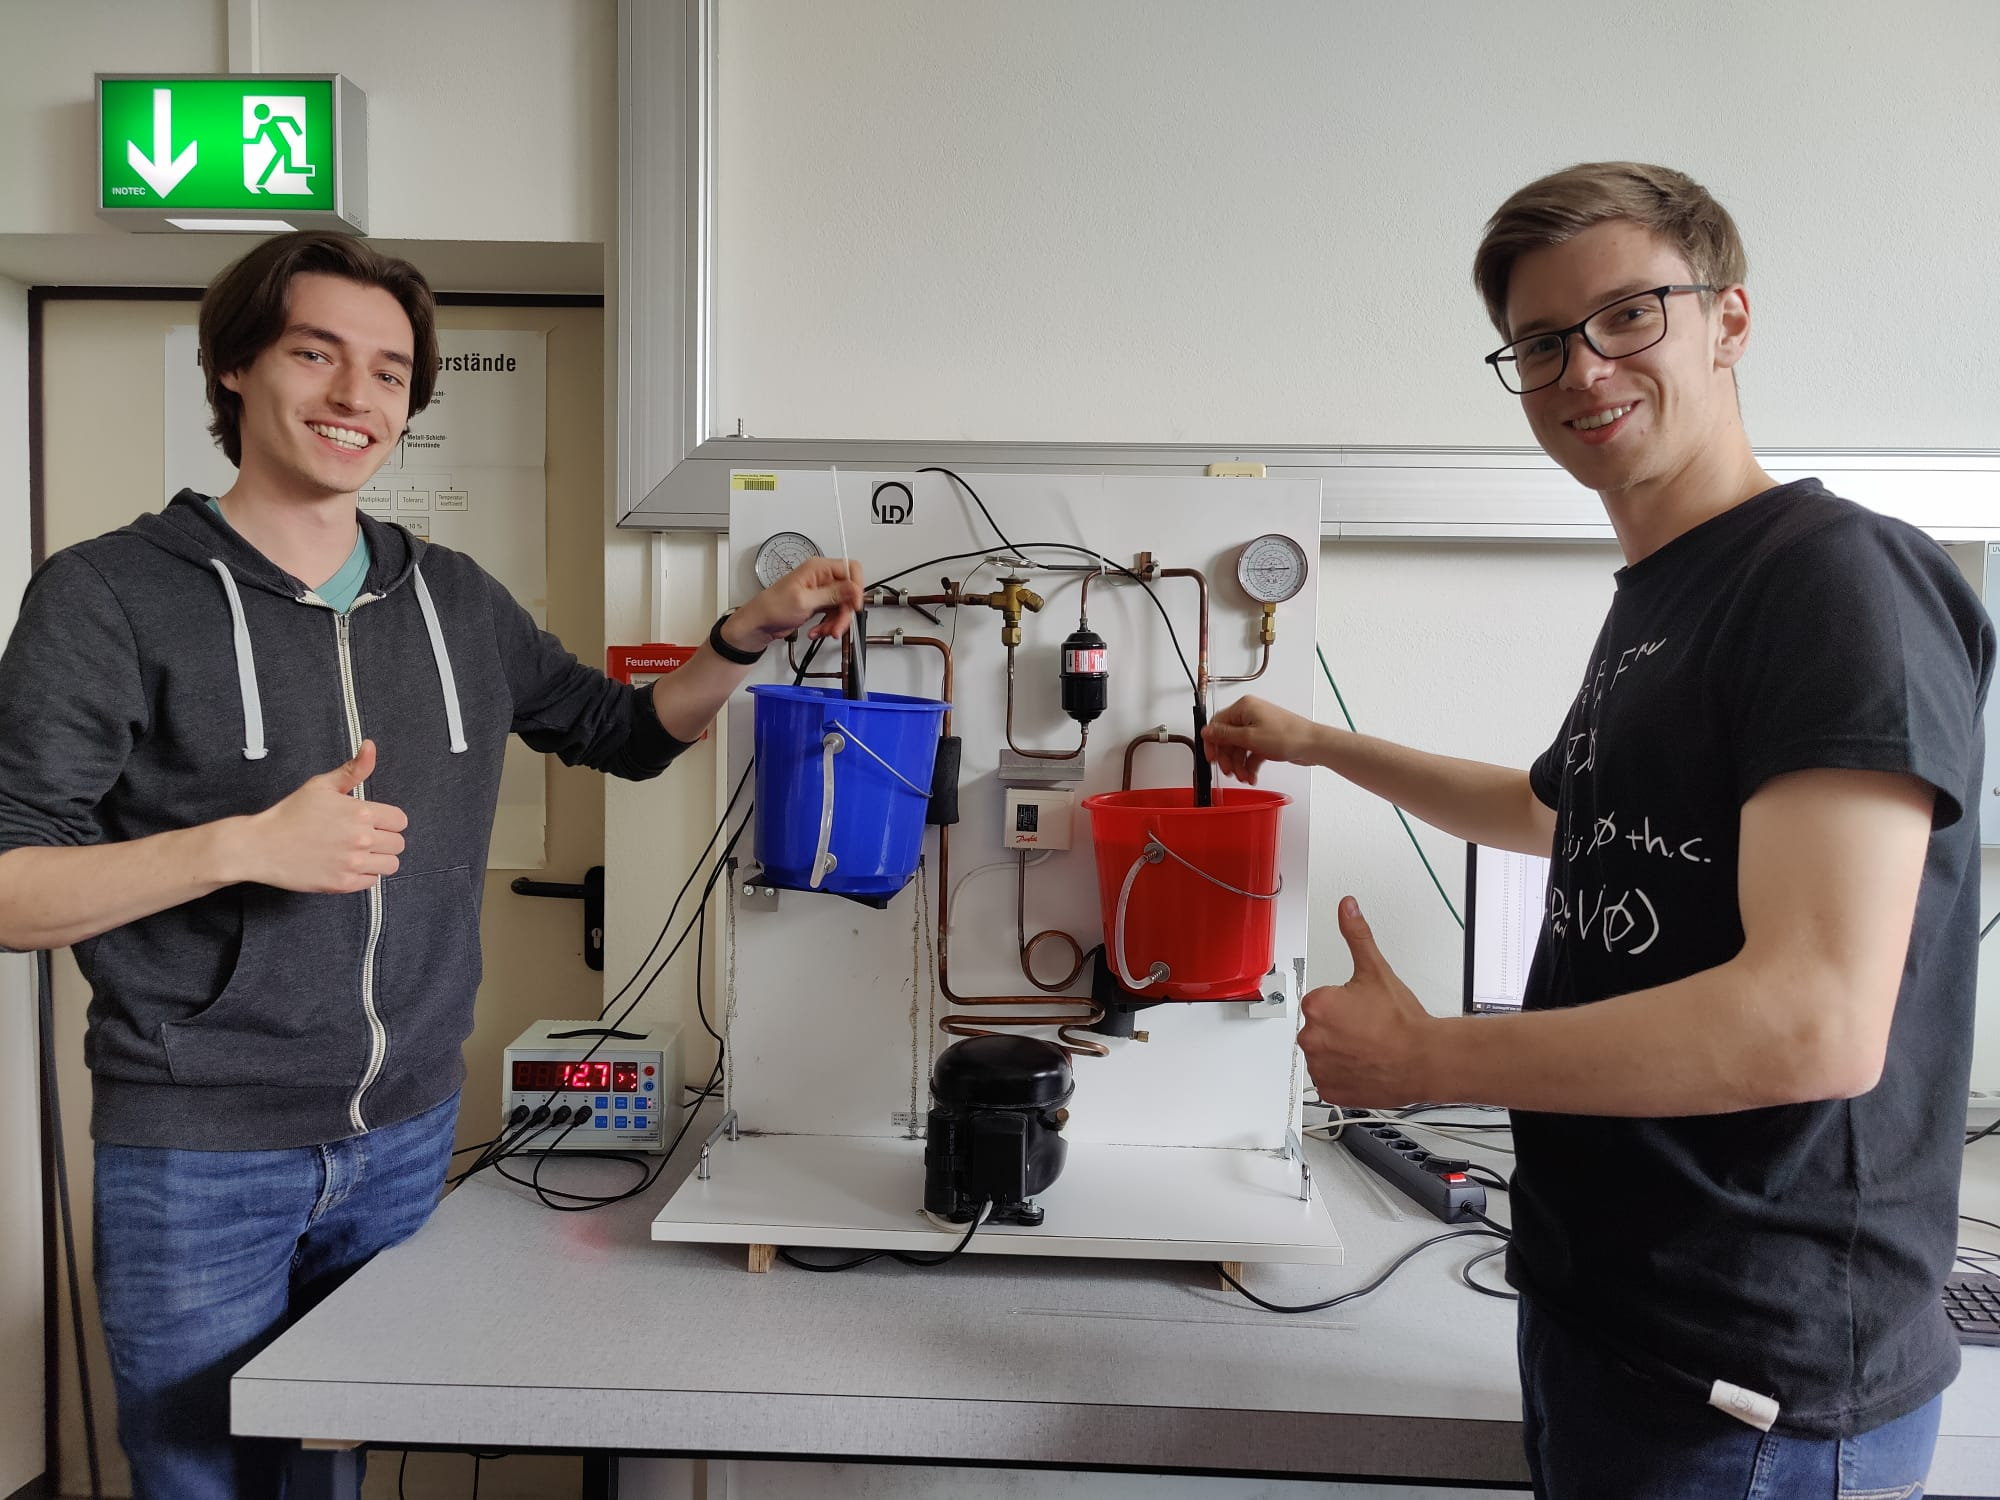
\includegraphics[width=0.6\linewidth]{fig/Spass1.jpeg}
        \caption[Symbolbild Experimentatoren]{Symbolbild Experimentatoren}
        \label{fig:umruehren}
    \end{samepage}
\end{figure}



\section{Auswertung}
\label{sec:auswertung}

\subsection{Solarzelle mit Lampe}
\label{subsec:auswertung_solar_lampe}

\subsection{Solarzelle mit Sonnensimulator}
\label{subsec:auswertung_solar_sonnensimulator}

\subsection{Wärmepumpe}
\label{subsec:auswertung_waermepumpe}

Die von Cassy-Lab2 erhaltenen Daten zu den beiden Temperaturkurven werden eingelesen und in \autoref{fig:plot_waermepumpe} dargestellt.

\begin{figure}[H]
    \centering
    \begin{samepage}
        \includegraphics[width=\linewidth]{}
        \caption[]{}
        \label{fig:}
    \end{samepage}
\end{figure}


\section{Diskussion}
% \label{sec:diskussion}
\subsection{Solarzelle}
\label{subsec:diskussion_solar}

\subsection{Wärmepumpe}
\label{subsec:diskussion_waermepumpe}


\section{Zusammenfassung}
\label{sec:zusammenfassung}


\clearpage
% Literaturverzeichnis
\printbibliography

% Abbildungsverzeichnis
\listoffigures

% Tabellenverzeichnis
\listoftables

\end{document}
